\documentclass[11pt]{amsart}
\usepackage{geometry}                % See geometry.pdf to learn the layout options. There are lots.
\geometry{letterpaper}                   % ... or a4paper or a5paper or ... 
%\geometry{landscape}                % Activate for for rotated page geometry
%\usepackage[parfill]{parskip}    % Activate to begin paragraphs with an empty line rather than an indent
\usepackage{graphicx}
\usepackage{amssymb}
\usepackage{epstopdf}
\usepackage{tikz}
\DeclareGraphicsRule{.tif}{png}{.png}{`convert #1 `dirname #1`/`basename #1 .tif`.png}

\title{Regional MOM6}
\author{Kate Hedstrom}
\author{Alistair Adcroft}
\author{Robert Hallberg}
\author{Enrique Curchitser}
\date{}                                           % Activate to display a given date or no date

\begin{document}
\maketitle
\section{Introduction}
\section{Methods}

The goal of this project is to add open boundary conditions (OBCs)
to MOM6 such that it can be used as a regional model. The open
boundaries can be placed anywhere on the model grid between q-points
on the Arakawa C grid, including but not limited to the domain
boundaries.  In fact, is is possible to create a staircase of open
boundary segments at an angle through the domain, such as seen in
figure \ref{fdomain}. In order to support this feature, it is
necessary that nothing outside of the open boundary is used in the
model timestepping. If halo points were used, then both segments 2
and 3 in Figure \ref{fhalo} would be trying to set properties at
point A.

\begin{figure}
\begin{center}
\setlength{\unitlength}{10mm}
\begin{picture}(8.5,5.5)(0,0)
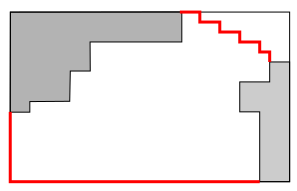
\includegraphics{pics/domain}
\end{picture}

\caption{An example of a domain with open boundary segments shown in red. Grey-shaded areas are land mask.}
\label{fdomain}
\end{center}
\end{figure}

\begin{figure}
\begin{center}
\setlength{\unitlength}{10mm}
%\begin{picture}
\begin{picture}(8,4.5)(0,0)

 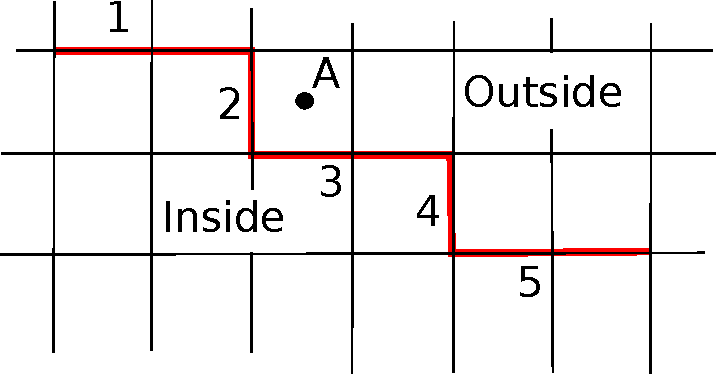
\includegraphics[width=8cm]{pics/halo}
\end{picture}
\caption{A portion of the grid with some numbered open boundary
segments. Point A is at a tracer point outside of OBC segments 2 and 3.}
\label{fhalo}
\end{center}
\end{figure}

\subsection{Barotropic}

\subsubsection{Specified}
For the barotropic mode, the only open boundary options are on the
velocity normal to a boundary segment. In the simplest case, one
knows both the barotropic velocity and the barotropic transport
through the OBC segments and can simply set them accordingly.

% Not sure what exact notation we want here.
\begin{equation}
  \overline{u}_{\rm seg} = \overline{u}
\end{equation}

\subsubsection{Flather}
\subsection{Normal velocity}
\subsubsection{Specified}
\subsubsection{Radiation}
\subsection{Tangential velocity}
\subsubsection{Vorticity}
\subsubsection{Strain}
\subsection{Tracers}
\section{Test problems}
\subsection{Barotropic Kelvin wave}
\subsection{Tracers}
\section{A realistic problem}
\section{Conclusions}
\section{Discussion}



\end{document}  
